%\renewcommand{\theequation}{\theenumi}
%\begin{enumerate}[label=\arabic*.,ref=\thesubsection.\theenumi]
%\numberwithin{equation}{enumi}

\item Find the equation of the circle with radius 5 whose centre lies on x-axis and passes through the point \myvec{2\\3}.
\\
\solution
Let $\vec{O}$ be the centre and $r$ be the radius of the given circle.
\\
$\therefore$
\begin{align}
    \label{eq:quad_form/2/1}
    \begin{split}
\vec{O} &= \myvec{p\\0}
\\
r &= 5
    \end{split}
\end{align}

The general equation of a circle is given by 
\begin{align}
\vec{x}^T\vec{x} - 2\vec{O}^T\vec{x} + \norm{\vec{O}}^2 -r^2 = 0
\end{align}
which, upon substitution from \eqref{eq:quad_form/2/1} yields
\begin{align}
\vec{x}^T\vec{x} - 2\myvec{p & 0}\vec{x} + p^2 - 25 = 0
\end{align}
$\because$
Point $\vec{A}$=\myvec{2\\3} lies on the circle, 
%
\begin{align}
\myvec{2 & 3}\myvec{2\\3} - 2\myvec{p & 0}\myvec{2\\3} + p^2 -25 &=0
\\
\implies p^2 - 4p - 12 &=0
\\
\implies p &=6 
\text{ or } -2
\end{align}

Hence,the possible equations of the circle are
\begin{align}
\vec{x}^T\vec{x} - 2\myvec{6 & 0}\vec{x} + 11 &= 0 \label{quad_form/2/1eq:1}
\\
\text{or}, \vec{x}^T\vec{x} - 2\myvec{-2 & 0}\vec{x} - 21 &= 0 \label{quad_form/2/1eq:2}
\end{align}

which are plotted in Fig. \ref{quad_form/2/1fig:circle}	


\begin{figure}[!ht]
\centering
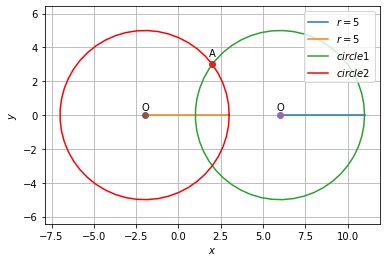
\includegraphics[width=\columnwidth]{solutions/su2021/2/1/Figure5.png}
\caption{Circles with centres (6,0) and (-2,0) respectively }
\label{quad_form/2/1fig:circle}	
\end{figure}



\item Find the equation of the circle passing through \myvec{0\\0} and making intercepts a and b on the coordinate axes.
\item Find the equation of a circle with centre \myvec{2\\2} and passes through the point \myvec{4\\5}. 
\item Find the locus of all the unit vectors in the xy-plane.
%
\item Find the points on the curve $\vec{x}^T\vec{x}-2\myvec{1 & 0}\vec{x} -3 =0$  at which the tangents are parallel to the x-axis.
%
\item  Find the area of the region in the first quadrant enclosed by x-axis, line $\myvec{1 & -\sqrt{3}}\vec{x} =0$ and the circle $\vec{x}^T\vec{x}=4$.
%
\item Find the area lying in the first quadrant and bounded by the circle $\vec{x}^T\vec{x}=4$ and the lines $x = 0$ and $x = 2$.
%
\item Find the area of the circle $4\vec{x}^T\vec{x}=9$.
\item  Find the area bounded by curves $\norm{\vec{x}-\myvec{1\\0}} = 1$ and $\norm{\vec{x}}=1$
\item Find the smaller area enclosed by the circle $\vec{x}^T\vec{x}=4$ and the line $\myvec{1 & 1}\vec{x} = 2$.
%\item The sum of the perimeter of a circle and square is $k$, where $k$ is some constant. Prove that the sum of their areas is least when the side of square is double the radius of the circle.
%\item A window is in the form of a rectangle surmounted by a semicircular opening. The total perimeter of the window is 10 m. Find the dimensions of the window to admit maximum light through the whole opening.
%
\item If 
$
\brak{x-a}^2+\brak{y-b}^2 = c^2,
$
for some $c > 0$, prove that 
\begin{align}
\frac{\brak{1+y_2}^\frac{3}{2}}{y_2}
\end{align}
%
is a constant independent of $a$ and $b$.
%
\item Form the differential equation of the family of circles touching the y-axis at origin.
\item Form the differential equation of the family of circles having centre on y-axis and radius 3 units.
\item Form the differntial equation of the fmaily of circles touching the x-axis at the origin.
%
\item Form the differential equation of the family of circles in the second quadrant and touching the coordinate axes.
\item Factorise $6x^2+ 17x + 5$.
\\
\solution 

The given polynomial can be expressed as:
\begin{align}
\vec{x}^T \myvec{6 & 0\\0 & 0}\vec{x}+ \myvec{17 & 0}\vec{x}+5=0
\end{align}
Substituting y=0 in the above equation,
\begin{align}
 6x^2+17x+5 &=0\\
\implies x&=\frac{-1}3{},\frac{-5}{2}\\
\therefore (3x+1)(2x+5) &=6x^2+17x+5
\end{align}
%
which is verified in Fig.     \ref{quadform/16/Fig:Graph Of $x^2+7x+10 &=$.}

\begin{figure}[ht!]
    \centering
    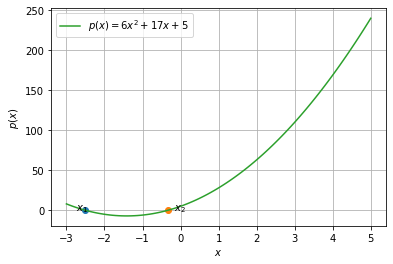
\includegraphics[width=\columnwidth]{solutions/su2021/2/16/Graph.png}
    \caption{Graph of $6x^2+17x+5$.}
    \label{quadform/16/Fig:Graph Of $x^2+7x+10 &=$.}
\end{figure}



\item Factorise $y^2 – 5y + 6$.
\item Find the zeroes of the quadratic polynomial $x^2+7x+10$ and verify the relationship between the zeroes and the coefficients.
\item Find the zeroes of the polynomial $x^2-3$ and verify the relationship between the zeroes and the coefficients.
\item Find a quadratic polynomial, the sum and product of whose zeroes are – 3 and 2, respectively.
%
\item Find the roots of the equation $5x^2  – 6x – 2 = 0 $.
\item Find the roots of $4x^2 + 3x + 5 = 0 $.
\item Find the roots of the following quadratic equations, if they exist.
\begin{enumerate}
\item 	$3x^2-5x+2 = 0$
\item 	$x^2+4x+5 = 0$
\item 	$2x^2-2\sqrt{2}x+1 = 0$
\end{enumerate}
%
\item Find the discriminant of the quadratic equation $2x^2-4x+3 = 0$
hence find the nature of its roots.
\\
\solution
We obtain the vertices of the rhombus as follows
\begin{align}
\vec{A} = \myvec{-3\\0},
\vec{B} = \myvec{0\\-3.5},
\vec{C} = \myvec{3\\0},
\vec{D} = \myvec{0\\3.5}
\end{align}
which are plotted in Fig. \ref{quad/45/fig:Rhombus ABCD}.
%
\begin{figure}[ht!]
\centering
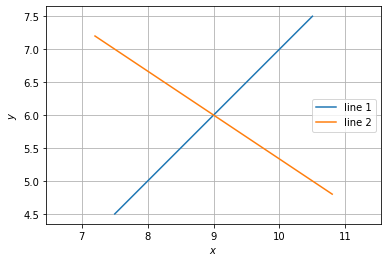
\includegraphics[width=\columnwidth]{solutions/quad/45/figure2.png}
\caption{Rhombus ABCD}
\label{quad/45/fig:Rhombus ABCD}
\end{figure}

\item Find the discriminant of the quadratic equation $3x^2-2x+\frac{1}{3} = 0$
hence find the nature of its roots.
\item Solve $x^2+ 2 = 0 $.
\item Solve $x^2+ x+1 = 0 $.
\item Solve $\sqrt{5}x^2+ x+\sqrt{5} = 0 $.
%
\item Find the coordinates of the focus, axis, the equation of the directrix and latus rectum of the parabola $y^2 = 8x$.
%
\item Find the equation of the parabola with focus \myvec{2\\0} and directrix $\myvec{1 & 0}\vec{x} = -2$.\item Find the equation of the parabola with vertex at \myvec{0\\ 0} and focus at \myvec{0\\ 2}.
\\
\solution
The equation of the plane is given by 
\begin{align}
\vec{n}^T\brak{\vec{x}-\vec{A}} &= 0
\\
\implies \myvec{1 & 1 & -1}{\vec{x}} &= \myvec{1 & 1 & -1}{\myvec{1\\0\\-2}}
\\
\text{or, }\myvec{1 & 1 & -1}{\vec{x}} &= 3
\end{align}
and plotted in Fig. \ref{linform/35/1/Plot of the plane}.

\begin{figure}[ht]
\centering
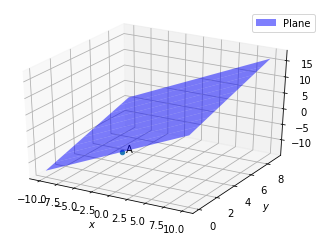
\includegraphics[width=\columnwidth]{solutions/su2021/2/35/1/Plane_plot1.PNG}
\caption{Plot of the plane}
\label{linform/35/1/Plot of the plane}
\end{figure}



\item Find the equation of the parabola which is symmetric about the y-axis, and passes through the point \myvec{2\\–3}.
\item Find the coordinates of the foci, the vertices, the length of major axis, the minor axis, the eccentricity and the latus rectum of the ellipse 
%
\begin{align}
\vec{x}^T\myvec{\frac{1}{25} & 0 \\ 0 & \frac{1}{9}}\vec{x} = 1
\end{align}
%
\item Find the coordinates of the foci, the vertices, the lengths of major and minor axes and the eccentricity of the ellipse 
%
\begin{align}
\vec{x}^T\myvec{9 & 0 \\ 0 & 4}\vec{x} = 36
\end{align}
%
\item Find the equation of the ellipse whose vertices are $\myvec{\pm 13\\ 0}$ and foci are $\myvec{\pm 5\\ 0}$.
%
\item Find the equation of the ellipse, whose length of the major axis is 20 and foci are $\myvec{0\\ \pm 5}$
%
\item Find the equation of the ellipse, with major axis along the x-axis and passing through the points \myvec{4\\ 3} and \myvec{– 1\\4}.
\\
\solution
Let 
\begin{align}
\vec{p} = \myvec{4\\3} , \vec{q} = \myvec{– 1\\4}
\end{align}
%
In general, the equation of the ellipse passing through $\vec{p}, \vec{q}$ can be expressed as
\begin{align}
\brak{\vec{x}-\vec{c}}^{\top}\vec{D}\brak{\vec{x}-\vec{c}}=1\label{quadforms/37/eq:14}
\end{align}
where the center $\vec{c}=\myvec{\beta\\0}$ and 
 $\vec{D}$ is a diagonal matrix.
$\because \vec{p}, \vec{q}$ satisfy \eqref{quadforms/37/eq:14},
\begin{align}
\label{quadforms/37/eq:ellipse_std_ab}
(\vec{p}-\vec{c})^{\top}\vec{D}(\vec{p}-\vec{c}) &= 1,
\\
(\vec{q}-\vec{c})^{\top}\vec{D}(\vec{q}-\vec{c}) &= 1,
\end{align}
which can be simplified as 
\begin{align}
    2\brak{\vec{p}-\vec{q}}^{\top}\vec{D}\vec{c}=\vec{p}^{\top}\vec{D}\vec{p}-\vec{q}^{\top}\vec{D}\vec{q}
\end{align}
Using the identity, 
\begin{multline}
    \brak{\vec{p}-\vec{q}}^{\top}\vec{D}(\vec{p}+\vec{q})
   =\vec{p}^{\top}\vec{D}\vec{p}-\vec{q}^{\top}\vec{D}\vec{q}
\end{multline}
in the above, 
\begin{multline}
    2\brak{\vec{p}-\vec{q}}^{\top}\vec{D}\vec{c}  = \brak{\vec{p}-\vec{q}}^{\top}\vec{D}(\vec{p}+\vec{q})
    \\
    \implies \brak{\vec{p}-\vec{q}}^{\top}\vec{D}\brak{2\vec{c}-\brak{\vec{p}+\vec{q}}} = 0
\end{multline}
Thus, $\vec{c}$ can be expressed in parametric form as 
\begin{align}
    \vec{c}=\frac{1}{2}\sbrak{\vec{p}+\vec{q}+ k\vec{D}^{-1}\vec{m}}
    \label{quadform/37/centre}
    \end{align}
    where 
\begin{align}
    (\vec{p}-\vec{q})^{\top}\vec{m}=0
    \label{quadform/37/dir}
\end{align}
and $k$ is a constant.  Substituting numerical values in     \eqref{quadform/37/dir},
\begin{align}
    \vec{p}-\vec{q} &= \myvec{5 \\ -1}
    \implies \vec{m} = \myvec{1 \\ 5}
\end{align}
Also, 
\begin{align}
    \vec{p}+\vec{q} &= \myvec{3 \\ 7}
\end{align}
which, upon substitution in     \eqref{quadform/37/centre} yields 
\begin{align}
 \myvec{\beta\\0}=\frac{1}{2}\sbrak{\myvec{3\\7}+k\myvec{\frac{1}{\lambda_1} & 0 \\ 0 & \frac{1}{\lambda_2}}\myvec{1\\5}}
\end{align}
From the given information, the $X-$axis is the major axis.  Hence, 
\begin{align}
    \frac{\lambda_2}{\lambda_1}>1
    \implies \frac{2\beta-3}{\frac{-7}{5}}>1\\
    \text{or, } \beta<0.8
\end{align}
%
The possible ellipses satisfying the above condition are plotted in Fig. \ref{quadforms/37/fig:ellipses}.	
\begin{figure}[!ht]
\centering
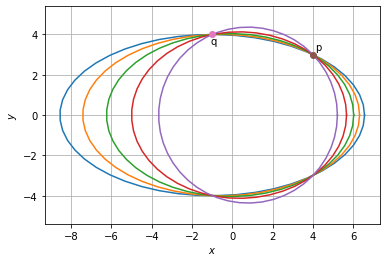
\includegraphics[width=\columnwidth]{solutions/su2021/2/37/figure5_1.png}
\caption{Ellipses passing through the two points with X axis as major axis}
\label{quadforms/37/fig:ellipses}	
\end{figure}
%

%
\item Find the coordinates of the foci and the vertices, the eccentricity,the length of the latus rectum of the hyperbolas
\begin{enumerate}
\item 
$
\vec{x}^T\myvec{\frac{1}{9} & 0 \\ 0 & -\frac{1}{16}}\vec{x} = 1
$
\item 
$
\vec{x}^T\myvec{1 & 0 \\ 0 & -16}\vec{x} = 16
$
\end{enumerate}
\solution
\begin{enumerate}
    \item 

The total amount spent is given by=

    \begin{multline}
    \vec{B}\vec{A}\\
    =\myvec{1000&500&5000\\3000&1000&10000}\myvec{40\\100\\50}\\
    =\myvec{40000+50000+250000\\120000+100000+500000}\\
    \begin{blockarray}{cc}
    \text{TotalCost} \\
    \begin{block}{(c)(c)}
    340000&\text{X}\\
    720000&\text{Y}\\
    \end{block}
    \end{blockarray}
    \end{multline}
$\therefore$ the total amount spent in city X and city Y is 3400 and 7200 Rupees respectively.  See Fig. \ref{matrix/64fig:Profit}	
%
\begin{figure}[!ht]
\centering
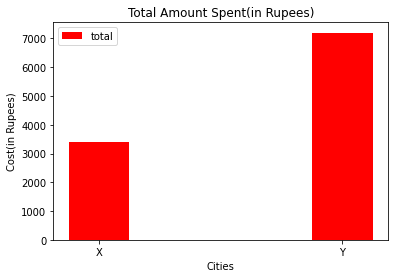
\includegraphics[width=\columnwidth]{solutions/su2021/64/figure8.png}
\caption{Total Amount Spent by the group in cities X and Y}
\label{matrix/64fig:Profit}	
\end{figure}

\end{enumerate}

\item Find the equation of the hyperbola with  vertices $\myvec{0 \\ \pm \frac{\sqrt{11}}{2}}$, foci $\myvec{ 0\\ \pm 3}$
\item Find the equation of the hyperbola with   foci $\myvec{ 0\\ \pm 12}$ and length of latus rectum 36.
%
\item Find the equation of all lines having slope 2 and being tangent to the curve
\begin{align}
y + \frac{2}{x-3} = 0
\end{align}
%
\\
\solution

The equation of curve can be expressed as 
\begin{align}
  y+\frac{2}{x-3}=0  \\
  xy-3y+2=0\label{quadform/41/eq:giveneq}
\end{align}
Comparing with the standard equation, 
\begin{align}
\vec{x}^T\vec{V}\vec{x}+2\vec{u}^T\vec{x}+f=0\\
\vec{V}=\myvec{0&\frac{1}{2}\\\frac{1}{2}&0},\vec{u}=\myvec{0\\-\frac{3}{2}},f=2\\
\vec{V}^{-1}=\myvec{0&2\\2&0}
\end{align}
$\because$
\begin{align}
    \abs{\vec{V}} &= \frac{-1}{4}
    \\
    \implies \abs{\vec{V}} &< 0
\end{align}
and \eqref{quadform/41/eq:giveneq} represents a hyperbola.
The characteristic equation of $\vec{V}$ is 
\begin{align}
    \abs{\vec{V} - \lambda\vec{I}} = \mydet{-\lambda & \frac{1}{2} \\ \frac{1}{2} & -\lambda} &= 0
    \\
    \implies \lambda^2 - \frac{1}{4} &= 0
\end{align}
and the eigenvalues are 
\begin{align}
    \lambda_1 = \frac{1}{2} , \lambda_2 = \frac{-1}{2}
\end{align}
% Eigen vector $\vec{p}$ is 
% \begin{align}
%     \vec{V}\vec{p} &= \lambda\vec{p}
%     \\
%     \implies (\vec{V} - \lambda\vec{I})\vec{p} &= 0
% \end{align}
Eigen vector $\vec{p}_1$ corressponding to $\lambda_1$ can be obtained as
\begin{align}
    (\vec{V} - \lambda_1\vec{I}) &= \myvec{\frac{-1}{2} & \frac{1}{2} \\ \frac{1}{2} & \frac{-1}{2}}\xleftrightarrow[R_1 \leftarrow -2R_1]{R_2 = R_1 + R_2}\myvec{1 & -1 \\ 0 & 0}
    \\
    \implies \vec{p_1} &= \frac{1}{\sqrt{2}}\myvec{1 \\ 1}
\end{align}
Similarly,
\begin{align}
    \vec{p_2} &= \frac{1}{\sqrt{2}}\myvec{-1 \\ 1}
\end{align}
$\therefore$
\begin{align}
    \vec{P} &= \myvec{\vec{p_1} & \vec{p_2}} = \frac{1}{\sqrt{2}}\myvec{1 & -1 \\ 1 & 1}
    \\
    \vec{D} &= \myvec{\lambda_1 & 0 \\ 0 & \lambda_2} = \myvec{\frac{1}{2} & 0 \\ 0 & \frac{-1}{2}}
\end{align}
Now,
\begin{align}
    \vec{c} &= -\vec{V}^{-1}\vec{u} 
    \\
    &= -\myvec{0 & 2 \\2 & 0}\myvec{0 \\ \frac{-3}{2}}
    \\
    &= \myvec{3 \\ 0}
\end{align}
\begin{align}
\because \vec{u}^T\vec{V}^{-1}\vec{u} - f<0,
\end{align}
the axes need to be swapped and 
\begin{align}
    \sqrt{\frac{ \vec{u}^T\vec{V}^{-1}\vec{u} - f}{\lambda_2}} &= 2
    \\
    \sqrt{ \frac{f- \vec{u}^T\vec{V}^{-1}\vec{u}}{\lambda_1}} &= 2
\end{align}
$\therefore$ the equation of the standard hyperbola can be expressed as 
\begin{align}
    \frac{y^2}{4} - \frac{x^2}{4} &= 1
\end{align}
The direction and normal vectors of tangent with slope 2 are 
\begin{align}
    \vec{m}=\myvec{1\\2},\vec{n}=\myvec{-2\\1}
\end{align}
From the  conics table in the manual,
\begin{align}
\kappa = \pm \sqrt{\frac{\vec{u}^T\vec{V}^{-1}\vec{u}-f}{\vec{n}^T\vec{V}^{-1}\vec{n}}} = \pm \sqrt{\frac{1}{4}} = \pm \frac{1}{2}
\end{align}
and the desired points of contact are 
\begin{align}
\vec{q}&=\vec{V}^{-1}(\kappa\vec{n}-\vec{u})\\
\implies \vec{q}_1=\myvec{4\\-2}, 
\vec{q}_2=\myvec{2\\2}\label{quadform/41/eq:10}
\end{align}
The equation of the tangents are given by
\begin{align}
    \vec{n}^T\vec{x}&=\vec{n}^T\vec{q}\\
    \implies \myvec{-2&1}\vec{x}&=\myvec{-2&1}\myvec{4\\-2}=-10\\
    \text{and }\myvec{-2&1}\vec{x}&=\myvec{-2&1}\myvec{2\\2}=-2
\end{align}
%
The above results are verified in Fig. \ref{quadform/41/fig:tangents}.	
\begin{figure}[!ht]
\centering
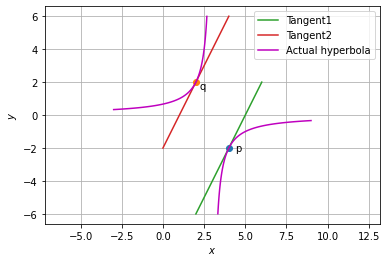
\includegraphics[width=\columnwidth]{solutions/su2021/2/41/figure6_1.png}
\caption{The tangents to the curve with slope 2 }
\label{quadform/41/fig:tangents}	
\end{figure}




\item Find the point at which the tangent to the curve $y = \sqrt{4x-3}-1$ has its 
slope $\frac{2}{3}$.
%
\\
\solution
Given curve,
\begin{align}
y = \sqrt{4x-3}-1\label{quadform/42/2.0.1}\\
\implies (y+1)^2 =4x-3\\
\implies y^2-4x+2y+4 =0
\end{align}
which has the vector parameters
\begin{align}
\vec{V}&=\myvec{0 & 0 \\ 0 & 1},\vec{u}=\myvec{-2 & 1 }, \vec{f} = 4 
\end{align}
\begin{align}
|\vec{V}| = 0
\end{align}
$\therefore $ the given curve \eqref{quadform/42/2.0.1} is parabola. In standard form,
\begin{align}
\vec{P} =\vec{I}\implies \vec{p_1} = \myvec{1 \\ 0}
\end{align}
Since the slope of the tangents is $\frac{2}{3}$, the direction and normal vectors are
\begin{align}
\vec{m} &= \myvec{1\\\frac{2}{3}}= \myvec{3\\2},\vec{n} = \myvec{2\\-3}\\
\text{and }
\kappa &= \frac{\vec{p_1^T}\vec{u}}{\vec{p_1^T}\vec{n}} = -1
\end{align}
$\therefore$ Point of contact for the tangent is
\begin{align}
  \myvec{\vec{u}+\kappa \vec{n^T}\\\vec{V} }\vec{q} &= \myvec{\vec{-f}\\\kappa \vec{n} -\vec{u}}\\
  \implies\myvec{-4 & 4\\0 & 0 \\0 & 1} \vec{q}&= \myvec{-4\\0\\2}\\
  \implies \vec{q}&=\myvec{3\\2}
\end{align}
%$\therefore $ Point of contact for tangent of given curve is
% \begin{align}
% \vec{q }= \myvec{3\\2}
% \end{align}
which is verified in Fig.     \ref{quadform/42/fig:Tangent to parabola.}
%
\begin{figure}[ht]
    \centering
    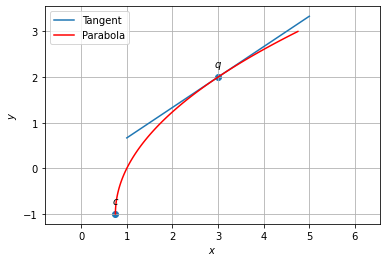
\includegraphics[width=\columnwidth]{solutions/su2021/2/42/PARABOLA.png}
    \caption{Tangent to Parabola.}
    \label{quadform/42/fig:Tangent to parabola.}
\end{figure}    




\item Find the roots of the following equations:
\begin{enumerate}
\item  $x + \frac{1}{x} = 3, x \ne =0 $
\item  $ \frac{1}{x} + \frac{1}{x-2}=3, x\ne =0, 2 $
\end{enumerate}
%
\item Find points on the curve 
$
\vec{x}^T\myvec{\frac{1}{4} & 0 \\ 0 & \frac{1}{25}}\vec{x} = 1
$
at which the tangents are 
\begin{enumerate}
\item parallel to x-axis
\item parallel to y-axis
\end{enumerate}
 \item Find the equation of the normal to the curve $x^2= 4y$
which passes through the point \myvec{1\\ 2}.
%
\solution
The given curve can be expressed as 
\begin{align}
 x^2-4y &=0 \label{quadform/45/2.0.2}
 \\
%\vec{x}^T\vec{V}\vec{x}+2\vec{u}^T\vec{x}+f=0\\
\implies \vec{V}=\myvec{1 & 0 \\ 0 & 0},\vec{u}=\myvec{0 \\ -2 }, \vec{f} = 0 
\end{align}
$\because$
\begin{align}
 \abs{\vec{V}} &= 0
\end{align}
the given curve \eqref{quadform/45/2.0.2} represents a parabola.
The eigenvalues are given by 
\begin{align}
\lambda_1 = 0 , \lambda_2 = 1
\end{align}
with corresponding eigenvectors
\begin{align}
\myvec{1 & 0 \\ 0 & 0}\vec{x} &=0 \implies \vec{p_1} = \myvec{0 \\ 1}
\\
\myvec{0 & 0 \\ 0 & -1}\vec{x} &=0 \implies \vec{p_2} = \myvec{1 \\ 0}
\end{align}
To find the vertex of the parabola ,
\begin{align} \myvec{\vec{u^T}+\kappa\vec{p_1^T}\\\vec{V} }\vec{c} &= \myvec{\vec{-f}\\\kappa \vec{p_1} -\vec{u}}
\\
\text{where, }  \kappa = \vec{u^T}\vec{p_1} = -2
\\
\implies\myvec{0 & -4\\1 & 0 \\0 & 0} \vec{c}&= \myvec{0\\0\\0} \label{quadform/45/eq:b}
\end{align}
from the above it can be observed that,
\begin{align}    
   \vec{c} &= \myvec{0 \\ 0}
\end{align}
Now to evalute the direction vector m,
\begin{align}
\vec{m}^T(\vec{V}\vec{q} + \vec{u}) &=0
\\
\implies \vec{m}^T\brak{\myvec{1 & 0 \\ 0 & 0}\myvec{1 \\ 2} + \myvec{0 \\ -2}} &=0
\\
\implies \vec{m}^T\myvec{1 \\ -2} &=0
\\
\implies \vec{m} = \myvec{-2 \\ -1}
\end{align}
The normal is obtained as 
\begin{align}
\vec{m}^T(\vec{x} - \vec{q}) &=0 
\\
\myvec{-2 & -1}\brak{\vec{x}-\myvec{1 \\ 2}} &= 0
\\
\myvec{-2 & -1}\vec{x}+ 4 &= 0 
\end{align}
%
The above results are verified in Fig.     \ref{quadform/45/fig:Normal to parabola.}.
\begin{figure}[ht]
    \centering
    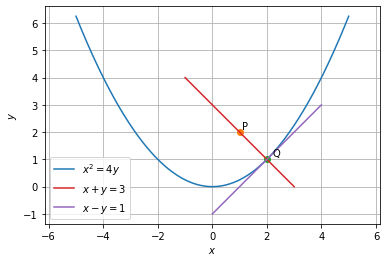
\includegraphics[width=\columnwidth]{solutions/su2021/2/45/FIGURE4.png}
    \caption{Normal to Parabola.}
    \label{quadform/45/fig:Normal to parabola.}
\end{figure}    


%
\item Find the area enclosed by the ellipse
$
\vec{x}^T\myvec{\frac{1}{a^2} & 0 \\ 0 & \frac{1}{b^2}}\vec{x} = 1
$
%
\item Find the area of the region bounded by the curve $y = x^2$
and the line $y = 4$.
%
\item Find the area bounded by the ellipse
$
\vec{x}^T\myvec{\frac{1}{a^2} & 0 \\ 0 & \frac{1}{b^2}}\vec{x} = 1
$
and $x = ae$, where, $b^2 = a^2 (1 – e^2 )$ and $e < 1$.
%
\item Prove that the curves $y^2 = 4x$ and $x^2 = 4y$ divide the area of the square bounded by $x = 0, x = 4, y =4$ and $y = 0$ into three equal parts.
%
\item Find the area of the region
\begin{align}
\cbrak{\brak{x,y} = 0\le y\le x^2+1, 0\le y \le x+1, 0 \le x \le 2}
\end{align}
\item Find the intervals in which the function 
\begin{align}
f(x)  = x^2-4x+6
\end{align}
%
is 
\begin{enumerate}
\item increasing
\item decreasing.
\end{enumerate}
%
%\item Find the shortest distance of the point $\myvec{0\\c}$ from the parabola $y = x^2$, where $\frac{1}{2} \le c \le 5$.
%
%\item An apache helicopter of enemy is flying along the curve given by $y = x^2+7$.  A soldier, placed at \myvec{3\\7}, wants to shoot down the helicopter when it is nearest to him.  Find  the nearest distance.
%
\item Examine whether the function $f$ given by $f(x) = x^2$ is continuous at $x = 0$.
%
\item Discuss the continuity of the function $f$ defined by 
%
\begin{align}
f(x)  = 
\begin{cases}
x & x \ge 0
\\
x^2 & x < 0
\end{cases}
\end{align}
%
\item Verify Rolle's theorem for the function $y = x^2+2, a = -2$ and $b = 2$.
\item Verify Mean Value Theorem for the function $f(x) = x^2$ in the interval $\sbrak{2,-4}$.
%\end{align}
\item Find the derivative of $f(x) = x^2$.
\item Find the derivative of $ x^2 - 2$ at $x = 10$.
\item Find the derivative of $ \brak{x-1} \brak{x-2}$.
%
%
\item Find 
\begin{align}
\int_{0}^{2} \brak{x^2+1}\,dx
\end{align}
%
as a limit of a sum.
\item Evaluate the following integral:
%
\begin{align}
\int_{2}^{3}x^2 \,dx
\end{align}
%
\item Form the differntial equation representing the family of ellipses having foci on x-axis and cenre at the origin.
%
\item Form the differntial equation representing the family of parabolas having vertex at origin and axis along positive direction of x-axis.
\item Form a differntial equation representing the following family of curves
%
\begin{align}
y^2 = a\brak{b^2-x^2}
\end{align}
%
\item  A cricket ball is thrown at a speed of 28 $m s^{-1}$
in a direction 30$\degree$ above
the horizontal. Calculate 
\begin{enumerate}
\item  the maximum height, 
\item  the time taken by the ball to return to the same level, and 
\item  the distance from the thrower to the point where the ball returns to the same level.
\end{enumerate}
\item Find the roots of the equation  $2x^2– 5x + 3 = 0$ .
\item Find the value of  the following polynomial at the indicated value of variables 
\begin{align}
p(x) = 5x^2– 3x + 7 \text{  at } x = 1.
\end{align}
%\end{enumerate}
